
% {
% \setbeamertemplate{headline}{}
% \setbeamertemplate{footline}{}
% \setbeamertemplate{navigation symbols}{}
% \begin{frame}
% \begin{block}{}
% \begin{quote}
% The only thing that is constant is change.\\
% \hfill Heraclitus of Ephesus
% \end{quote}
% \end{block}
% \end{frame}
% }

% \section{Introduction}
% \subsection{Motivation}
\begin{frame}{Motivation}%{A Sub-title is optional}
\begin{itemize}
\item Software applications change all the time
\item Deployed systems must be updated with bug fixes, new features
\item Updating typically involves: stop, apply patch, restart
% \vspace{1ex}
% \begin{center}\begin{Huge}Updating $\Rightarrow$ Downtime\end{Huge}\end{center}
\item Not desirable
  \begin{itemize}
    \item Safety concerns
    \item Revenue loss
    \item Inconvenience
  \end{itemize}
\end{itemize}
% \item Might not be affordable for some applications
%   \begin{itemize}
%   \item Applications that retain state that cannot be externalized
%   \end{itemize}
\end{frame}

\begin{frame}{Dynamic software updating}%{A Sub-title is optional}
\vspace*{-3mm}%
\begin{center}%
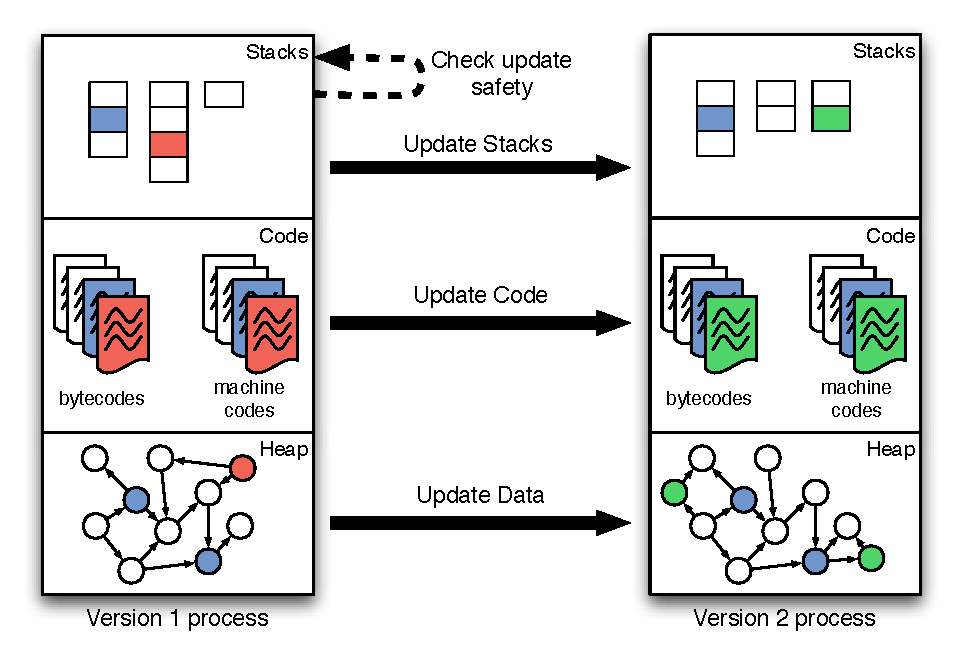
\includegraphics[scale=0.73]{images/process-state/both-process-state}%
\end{center}%
\end{frame}

\begin{frame}{Dynamic updating systems}%{A Sub-title is optional}
\begin{itemize}
\item Special-purpose architectures, application-specific solutions exist
\item General-purpose solutions gaining strength
  \begin{itemize}
  \item K42, Ksplice for OS updates
  \item Polus, Ginseng for C applications
  \end{itemize}
\item Not for managed languages
\end{itemize}
\end{frame}

% \begin{frame}{Motivation}%{A Sub-title is optional}
% \begin{itemize}
% \item Software applications change all the time
% \item Deployed systems need to be updated
% \item Some systems cannot afford downtime (safety concerns, revene loss),
% many systems perfer to avoid downtime (inconvenience)
% \item Stopping, updating and restarting deployed systems is not ideal
% \item Neither is delaying critical updates
% \end{itemize}
% \end{frame}

% \begin{frame}{Motivation}%{A Sub-title is optional}
% \begin{itemize}
% \item 75\% of downtime in high-availablity applications is for planned
% maintenance
% \uncover<2->{
% \item Personal operating system
% \item Enterprise applications
% \item Telecommunication, transportation systems
% % \uncover<3->{
% % \item Even a cache with lots of state
% %   \begin{itemize}
% %   \item LinkedIn.com architecture\footnote{\scriptsize{\url{http://hurvitz.org/blog/2008/06/linkedin-architecture}}}
% %   \item ``The Cloud'': In memory representation of the LinkedIn network graph
% %   \item Network size - 22M nodes, 120M edges
% %   \item Rebuilding an instance takes 8 hours
% %   \end{itemize}
% % }
% }
% \end{itemize}
% \end{frame}

% % \subsection{Solutions}
% \begin{frame}{Conventional solutions to avoid downtime}%{A Sub-title is optional}
% \begin{itemize}
% \item Move state out of the process, for instance databases
% \item Use multiple processes, and do a rolling update
% \end{itemize}
% \uncover<2>{
% \begin{itemize}
% \item Not always possible
% \item Restricted to specific application domains
% % \item DSU is a generic solution
% \end{itemize}
% }

% \begin{frame}{Dynamic Software Updating}%{A Sub-title is optional}
% Updating state of a process on the fly
% \begin{itemize}
% \item Special purpose techniques/architectures work, but we want a general
% solution
% \item 
% \end{itemize}
% \end{frame}

%   \begin{itemize}
%   \item State stored externally, for instance databases
%   \item Redundant systems: start a new process and stop this one
%   \item Not always possible
%   \end{itemize}
% \item<2-> Dynamic Software Updating (DSU)
%   \begin{itemize}
%     \item Update process state without restarting application
%     \item Non-redundant systems benefit as well
%     \item Decouples fault-tolerance from software updating
%   \end{itemize}
% \end{frame}

% \begin{frame}{Process state}%{A Sub-title is optional}
% \vspace*{-2ex}\includegraphics[scale=0.72]{images/process-state}
% \end{frame}

% \begin{frame}{DSU requirements}%{A Sub-title is optional}
% % \begin{center}
% % A Dynamic Software Updating solution should \emph{ideally} be
% % {\bf safe}, {\bf flexible}, and {\bf efficient}.
% % \end{center}
% \begin{description}
% \item[Safe] Updating is as correct as starting from scratch
% \item[Flexible] Support changes encountered in practice
% \item[Efficient] No performance impact
% \end{description}
% \end{frame}

% \begin{frame}{State of the art}%{A Sub-title is optional}
% Significant progress for C
% \begin{itemize}
% \item Server feature upgrades
%   \begin{itemize}
%   \item Ginseng \cite{neamtiu06dsu}
%   \item POLUS \cite{chen:icse07}
%   \end{itemize}
% \item Security patches: OPUS \cite{altekar05opus}
% \item Operating system upgrades
%   \begin{itemize}
%   \item K42 \cite{K42reconfig}
%   \item DynAMOS \cite{dynamos_eurosys_07}
%   \item LUCOS \cite{chen06vee}
%   \item Ksplice \cite{Ksplice}
%   \end{itemize}
% \end{itemize}
% % \item<2-> Primitive support for managed languages
% %   \begin{itemize}
% %   \item Very restrictive
% %   \item Space and time overheads
% %   \item Not proven on realistic applications
% %   \end{itemize}
% \end{frame}

% \begin{frame}{DSU opportunity for managed languages}%{A Sub-title is optional}
% DSU Solutions for C/C++ typically
% \begin{itemize}
% \item Require special compilation
% \item Statically/dynamically insert indirection for function calls
% \item Restrict structure updates, require extra allocation
% \item Impose space/time overheads on normal execution
% \item Make type-safety for updates difficult
% \item Not multi-threaded
% \end{itemize}
% \end{frame}

% \begin{frame}{Possible DSU solutions}%{A Sub-title is optional}
% Achieve DSU support by
% \begin{itemize}
% \item Making the application DSU-aware
% \item Special recompilation
% \item A class loader based colution 
% \item DSU support in the VM
% \end{itemize}
% \end{frame}

% \begin{frame}{Related work}%{A Sub-title is optional}
% \begin{itemize}
% \item Custom class loader solutions:\\Eisenbach and Barr, Milazzo et al.
% \item Source-to-source translation: Orso et al.
% \item VM-based solutions: JDrums, Dynamic Virtual Machine (DVM)
% \item In a persistent object store: Boyapati et al.
% \end{itemize}
% \uncover<2>{
% \begin{itemize}
% \item Limited, not flexible
% \item Restricted data-transformation model (like requiring {\em encapsulation} based
% on {\em ownership types})
% \item Overhead during normal execution
% \end{itemize}
% }
% \end{frame}

% \begin{frame}{Existing solutions for managed languages}%{A Sub-title is optional}
% \begin{itemize}
% \item VM-based solutions
%   \begin{itemize}
%   \item JDrums \cite{ritzau00dynamic}, DVM \cite{Mala00a}
%   \item Not well evaluated
%   \item Provide an interface similar to \DSU{}
%   \item Perform lazy updates
%   \item Overheads during normal execution
%   \end{itemize}
% \item Standard VM with DSU support
%   \begin{itemize}
%   \item DJVCS \cite{BarrE03}, DUSC \cite{orso:java}, \cite{Milazzo05updates}
%   \item Special classloaders, compilers
%   \item Very restrictive
%   \item Space/time overheads
%   \end{itemize}
% \end{itemize}
% 
% \end{frame}

% \begin{frame}{Related work}%{A Sub-title is optional}
% Nobody can beat us.
% \end{frame}

\begin{frame}{Our solution}%{A Sub-title is optional}
\begin{itemize}
\item \DSU{} - a Java Virtual Machine with DSU support
% \item Built on top of Jikes RVM, a Java-in-Java VM
\item Key insight: Extend existing VM services
%   \begin{itemize}
%   \item Classloading
%   \item Bytecode verification%\footnote{Jikes RVM does not have a bytecode verifier}
%   \item Thread synchronization
%   \item JIT Compilation
%   \item On-stack replacement
%   \item Garbage collection
%   \end{itemize}
\item No DSU-related overhead during normal execution
\item Support updates to real world applications
\begin{block}{}
\emph{Dynamic software updating in managed languages can be achieved in a
{\bf safe}, {\bf flexible} and {\bf efficient} manner by naturally extending existing VM
services.}
\end{block}

\begin{block}{}
\emph{DSU support should be a standard feature of future VMs.}
\end{block}
\end{itemize}
\end{frame}

% \begin{frame}{Contribution}%{A Sub-title is optional}
% \setbeamercovered{invisible}
% \begin{block}{}
% \emph{Dynamic software updating in managed languages can be achieved in a
% {\bf safe}, {\bf flexible} and {\bf efficient} manner by naturally extending existing VM
% services.}
% \end{block}
% 
% \begin{block}<2->{Corollary}
% \emph{DSU support should be a standard feature of future VMs.}
% \end{block}
% \end{frame}
